%%%%%%%%%%%%%%%%%%%%%%%%%%%%% Define Article %%%%%%%%%%%%%%%%%%%%%%%%%%%%%%%%%%
\documentclass{article}
%%%%%%%%%%%%%%%%%%%%%%%%%%%%%%%%%%%%%%%%%%%%%%%%%%%%%%%%%%%%%%%%%%%%%%%%%%%%%%%

%%%%%%%%%%%%%%%%%%%%%%%%%%%%% Using Packages %%%%%%%%%%%%%%%%%%%%%%%%%%%%%%%%%%
\usepackage{geometry}
\usepackage{graphicx}
\usepackage{amssymb}
\usepackage{amsmath}
\usepackage{amsthm}
\usepackage{empheq}
\usepackage{multicol}
\usepackage{mdframed}
\usepackage{booktabs}
\usepackage{lipsum}
\usepackage{blindtext}
\usepackage{graphicx}
\usepackage{color}
\usepackage{psfrag}
\usepackage{pgfplots}
\usepackage{bm}


%%%%%%%%%%%%%%%%%%%%%%%%%%%%%%%%%%%%%%%%%%%%%%%%%%%%%%%%%%%%%%%%%%%%%%%%%%%%%%%

% Other Settings

%%%%%%%%%%%%%%%%%%%%%%%%%% Page Setting %%%%%%%%%%%%%%%%%%%%%%%%%%%%%%%%%%%%%%%
\geometry{a4paper}

%%%%%%%%%%%%%%%%%%%%%%%%%% Define some useful colors %%%%%%%%%%%%%%%%%%%%%%%%%%
\definecolor{ocre}{RGB}{243,102,25}
\definecolor{mygray}{RGB}{243,243,244}
\definecolor{deepGreen}{RGB}{26,111,0}
\definecolor{shallowGreen}{RGB}{235,255,255}
\definecolor{deepBlue}{RGB}{61,124,222}
\definecolor{shallowBlue}{RGB}{235,249,255}
%%%%%%%%%%%%%%%%%%%%%%%%%%%%%%%%%%%%%%%%%%%%%%%%%%%%%%%%%%%%%%%%%%%%%%%%%%%%%%%

%%%%%%%%%%%%%%%%%%%%%%%%%% Define an orangebox command %%%%%%%%%%%%%%%%%%%%%%%%
\newcommand\orangebox[1]{\fcolorbox{ocre}{mygray}{\hspace{1em}#1\hspace{1em}}}
%%%%%%%%%%%%%%%%%%%%%%%%%%%%%%%%%%%%%%%%%%%%%%%%%%%%%%%%%%%%%%%%%%%%%%%%%%%%%%%

%%%%%%%%%%%%%%%%%%%%%%%%%%%% English Environments %%%%%%%%%%%%%%%%%%%%%%%%%%%%%
\newtheoremstyle{mytheoremstyle}{3pt}{3pt}{\normalfont}{0cm}{\rmfamily\bfseries}{}{1em}{{\color{black}\thmname{#1}~\thmnumber{#2}}\thmnote{\,--\,#3}}
\newtheoremstyle{myproblemstyle}{3pt}{3pt}{\normalfont}{0cm}{\rmfamily\bfseries}{}{1em}{{\color{black}\thmname{#1}~\thmnumber{#2}}\thmnote{\,--\,#3}}
\theoremstyle{mytheoremstyle}
\newmdtheoremenv[linewidth=1pt,backgroundcolor=shallowGreen,linecolor=deepGreen,leftmargin=0pt,innerleftmargin=20pt,innerrightmargin=20pt,]{theorem}{Theorem}[section]
\theoremstyle{mytheoremstyle}
\newmdtheoremenv[linewidth=1pt,backgroundcolor=shallowBlue,linecolor=deepBlue,leftmargin=0pt,innerleftmargin=20pt,innerrightmargin=20pt,]{definition}{Definition}[section]
\theoremstyle{myproblemstyle}
\newmdtheoremenv[linecolor=black,leftmargin=0pt,innerleftmargin=10pt,innerrightmargin=10pt,]{problem}{Problem}[section]
%%%%%%%%%%%%%%%%%%%%%%%%%%%%%%%%%%%%%%%%%%%%%%%%%%%%%%%%%%%%%%%%%%%%%%%%%%%%%%%

%%%%%%%%%%%%%%%%%%%%%%%%%%%%%%% Plotting Settings %%%%%%%%%%%%%%%%%%%%%%%%%%%%%
\usepgfplotslibrary{colorbrewer}
\pgfplotsset{width=8cm,compat=1.9}
%%%%%%%%%%%%%%%%%%%%%%%%%%%%%%%%%%%%%%%%%%%%%%%%%%%%%%%%%%%%%%%%%%%%%%%%%%%%%%%

%%%%%%%%%%%%%%%%%%%%%%%%%%%%%%% Title & Author %%%%%%%%%%%%%%%%%%%%%%%%%%%%%%%%
\title{Taller de latex }
\author{Marcela Sabogal Guerrero}
%%%%%%%%%%%%%%%%%%%%%%%%%%%%%%%%%%%%%%%%%%%%%%%%%%%%%%%%%%%%%%%%%%%%%%%%%%%%%%%

\begin{document}
    \maketitle
    \begin{abstract}
        \lipsum[3]
    \end{abstract}

 \section{Introducción}

\lipsum[2]
\cite{schmidt2020nonparametric}
\lipsum[2]
\cite{rasamoelina2020review}
 \section{Metodología}
\begin{multicols}{2}
    [ Esta es una prueba de \LaTeX para la charla con los MLSA $<3$]
    \blindtext
\end{multicols}
\lipsum[1]

Quiero referencia mi matrix \ref{matrix}, ahora mi fracción \ref{mifraccion}
\begin{figure}
    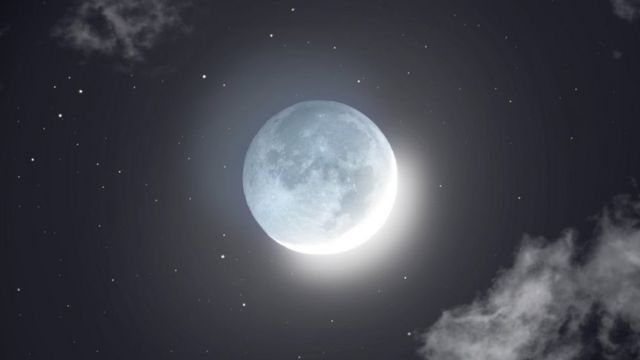
\includegraphics[width=\linewidth]{build/img/luna.jpg}
\end{figure}

\begin{table}[]
    \begin{tabular}{|c|c|c|c|c|}
    \hline
    \textbf{Números} & \textbf{rf} & \textbf{gr} & \textbf{fg} & \textbf{5}  \\ \hline
    \textbf{1}       & \textbf{2}  & \textbf{3}  & \textbf{4}  & \textbf{5} \\ \hline
    \textbf{4}       & \textbf{5}  & \textbf{6}  & \textbf{7}  & \textbf{7} \\ \hline
    \textbf{7}       & \textbf{6}  & \textbf{5}  & \textbf{34} & \textbf{6} \\ \hline
    \end{tabular}
    \end{table}
    \begin{table}[]
        \begin{tabular}{|c|c|c|c|c|}
        \hline
        \textbf{Números} & \textbf{rf} & \textbf{gr} & \textbf{fg} & \textbf{5}  \\ \hline
        \textbf{1}       & \textbf{2}  & \textbf{3}  & \textbf{4}  & \textbf{5} \\ \hline
        \textbf{4}       & \textbf{5}  & \textbf{6}  & \textbf{7}  & \textbf{7} \\ \hline
        \textbf{7}       & \textbf{6}  & \textbf{5}  & \textbf{34} & \textbf{6} \\ \hline
        \end{tabular}
        \end{table}    

\begin{equation} \label{matrix}
    \begin{bmatrix}
        3&3  & 4\\ 
        4& 5 & 5\\ 
        6& 65 & 5
    \end{bmatrix}    
\end{equation}
\begin{equation} \label{mifraccion}
   \left( \frac{2}{4}x + \frac{7}{8}\right)x=0   
\end{equation}


 \section{conclusión}

\begin{table}[]
    \begin{tabular}{|c|c|c|c|c|}
    \hline
    \textbf{Números} & \textbf{rf} & \textbf{gr} & \textbf{fg} & \textbf{5}  \\ \hline
    \textbf{1}       & \textbf{2}  & \textbf{3}  & \textbf{4}  & \textbf{5} \\ \hline
    \textbf{4}       & \textbf{5}  & \textbf{6}  & \textbf{7}  & \textbf{7} \\ \hline
    \textbf{7}       & \textbf{6}  & \textbf{5}  & \textbf{34} & \textbf{6} \\ \hline
    \end{tabular}
    \end{table}   
    \lipsum
\begin{figure}
    
\includegraphics[width=\linewidth]{build/img/logogit.jpg}
\caption{Imagen git}
\end{figure}


\bibliographystyle{ieeetr}
\bibliography{biliografia}

\end{document}